% KAJIAN PUSTAKA 2

\begin{frame}
    \begin{columns}
        \begin{column}{0.35\textwidth}
            \LARGE
            Kajian Pustaka 2
        \end{column}
        \begin{column}{0.6\textwidth}
            \justifying
            \textbf{Judul:}\\
            Spatial Attention fusion for obstacle detection using mmwave radar and vision sensor

            \vspace{1.5em}

            \textbf{Penulis:}\\
            Chang, Shuo; Zhang, Yifan; Zhang, Fan; Zhao, Xiaotong; Huang, Sai; Feng, Zhiyong; Wei, Zhiqing

            \vspace{1.5em}
            
            \textbf{Publikasi:}\\
            MDPI Sensors, vol.20, no.4, p.956, 2020
        \end{column}
    \end{columns}
\end{frame}


\begin{frame}
    \frametitle{Pustaka 2: Pendahuluan}
    \large
    \begin{itemize}
        \justifying
        \item mengintegrasikan Radar mmWave dengan Kamera untuk mendapatkan hasil deteksi halangan menggunakan metode Spatial Attention Feature (SAF)
        \vspace{1em}
        \item Mendapatkan hasil deteksi halangan yang lebih baik dibandingkan hanya menggunakan kamera atau radar
    \end{itemize}
\end{frame}


\begin{frame}
    \frametitle{Pustaka 2: Skema Sistem}
    \centering
        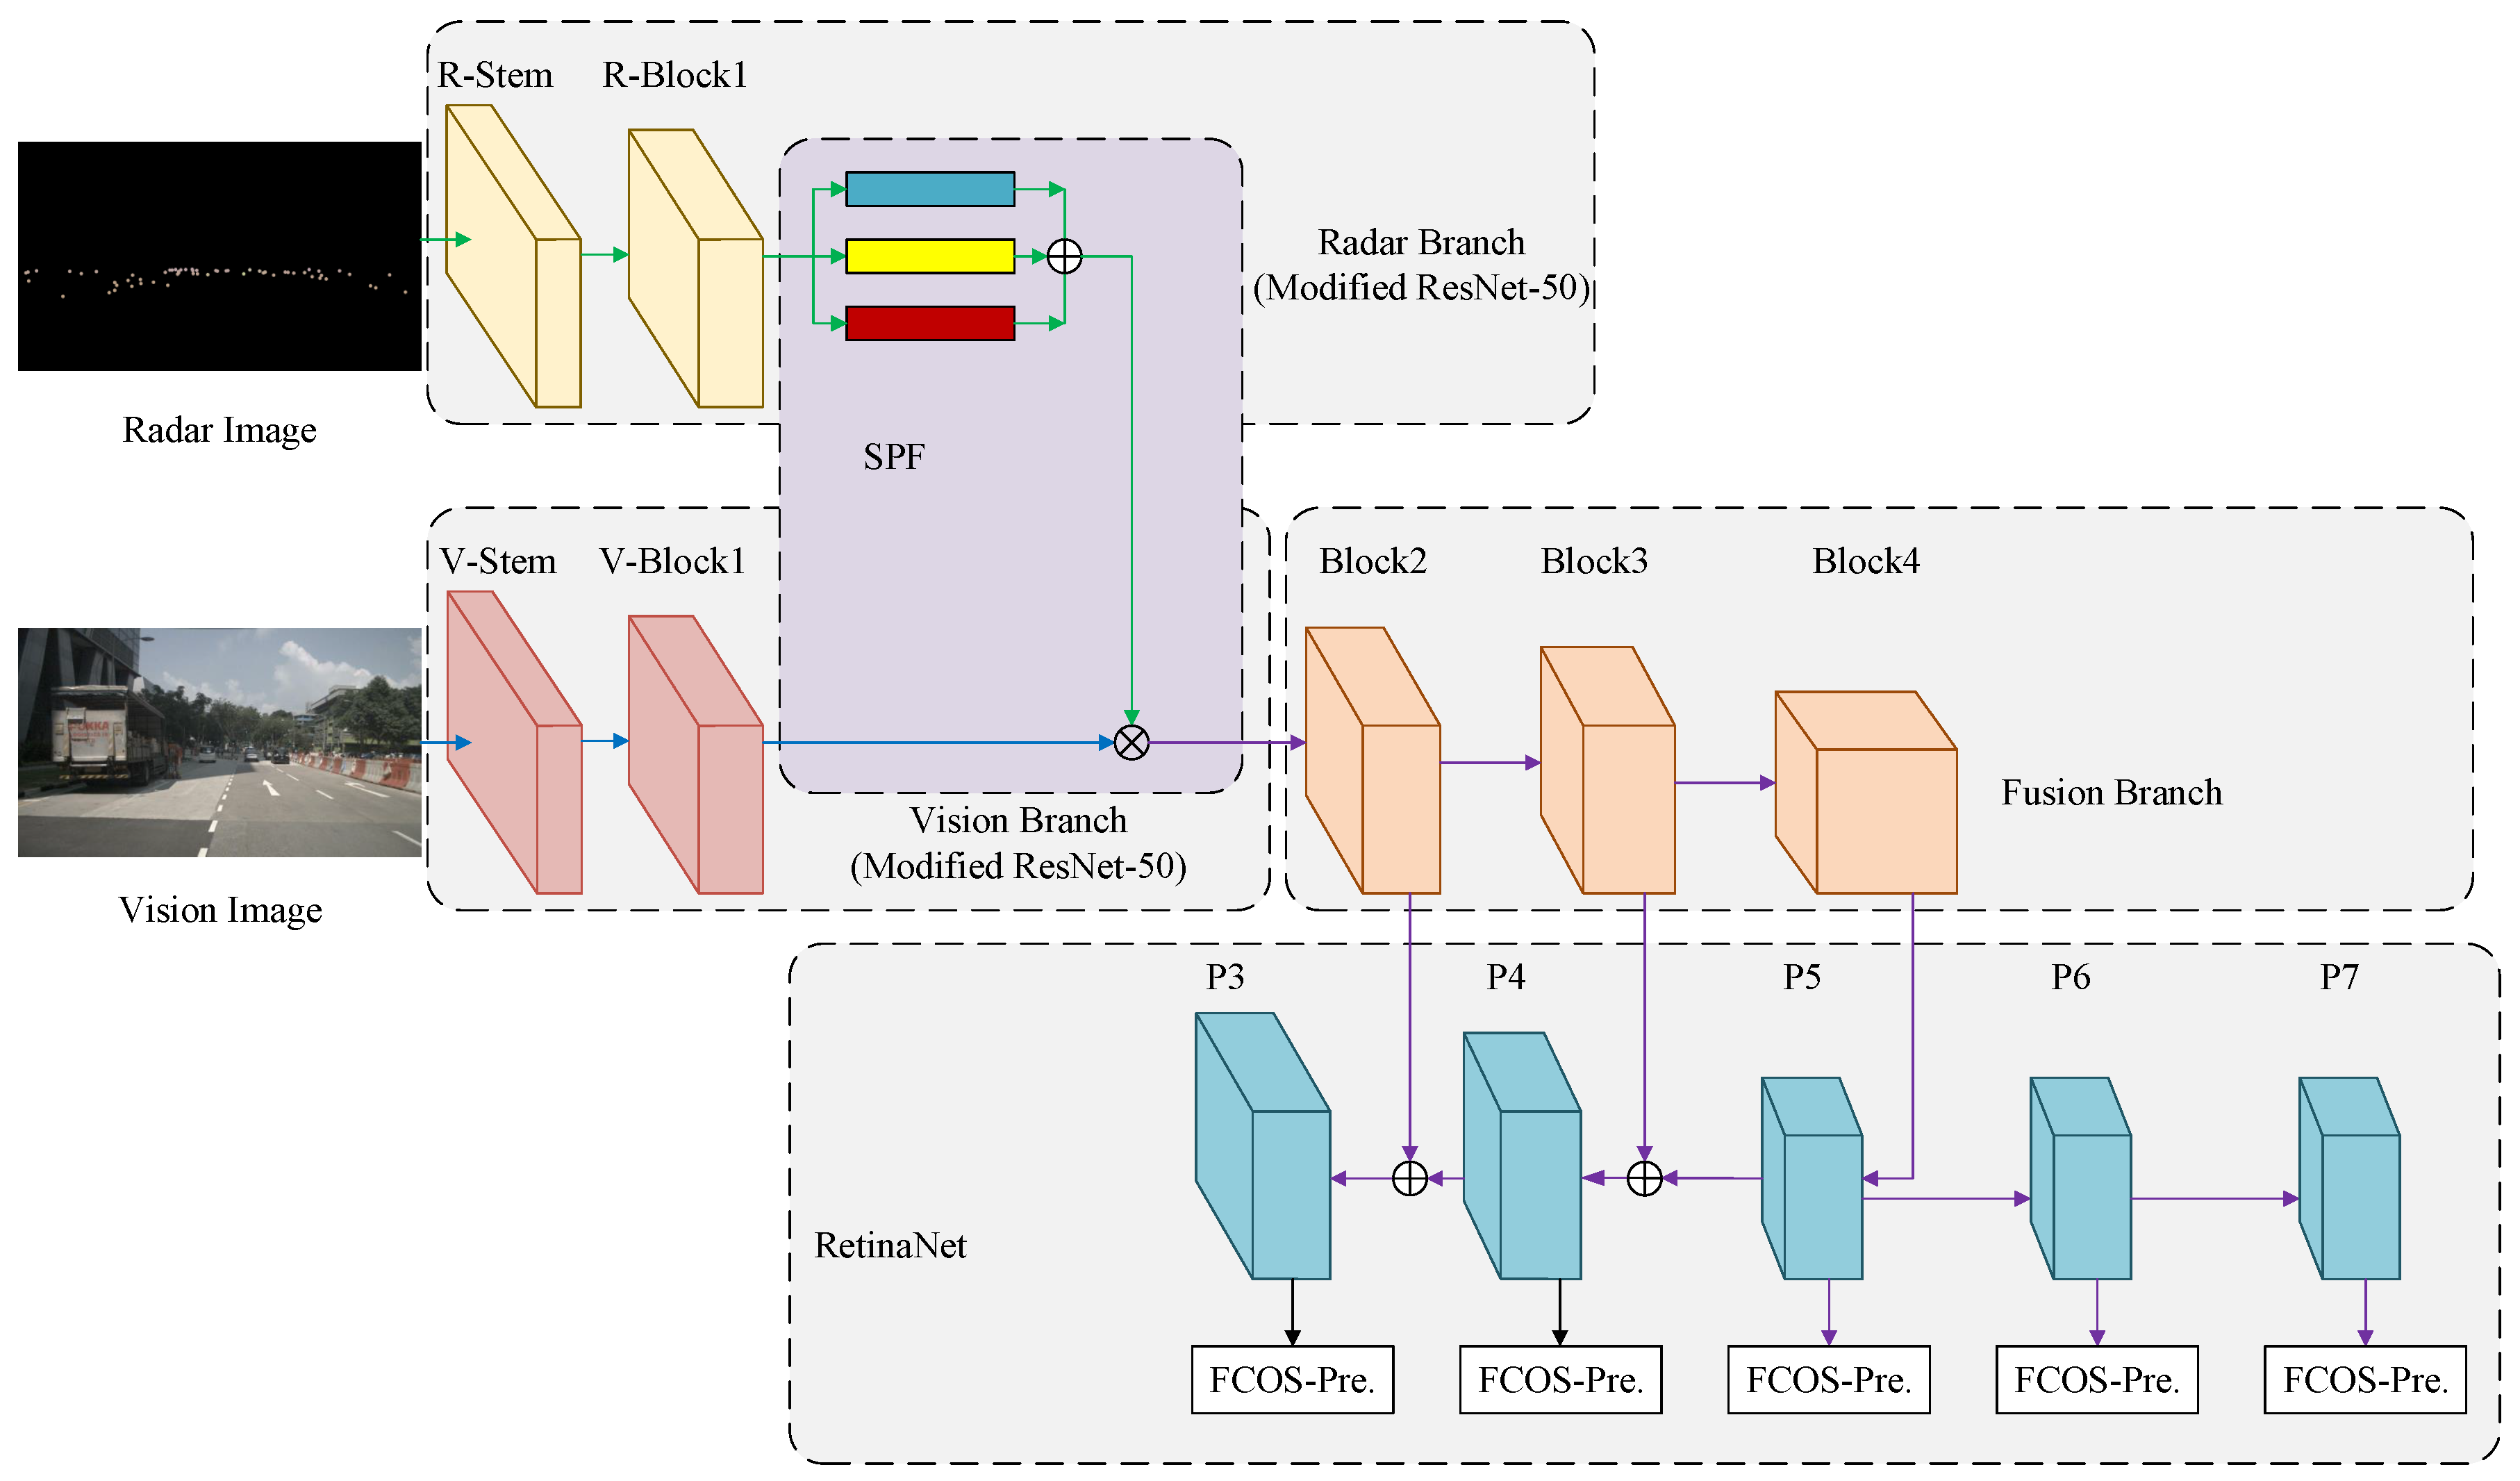
\includegraphics[width=.6\textwidth]{2-SAF-diagram.png}
\end{frame}


\begin{frame}
    \frametitle{Pustaka 2: Metode}
    \begin{enumerate}
        \justifying
        \item Deteksi Fitur Gambar dan Radar dengan ResNet50
        \item Fitur radar dimasukkan ke blok SAF/SPF
        \item Keluaran SAF dan Gambar digabungkan dengan Fusion Branch berbasis ResNet50
        \item Penentuan posisi dengan pyramid network RetinaNet
    \end{enumerate}
\end{frame}


\begin{frame}
    \frametitle{Pustaka 2: Hasil}
    \centering
    \includegraphics[width=\textwidth]{r2-hasil-1.png}
\end{frame}


\begin{frame}
    \frametitle{Pustaka 2: Hasil}
    \centering
    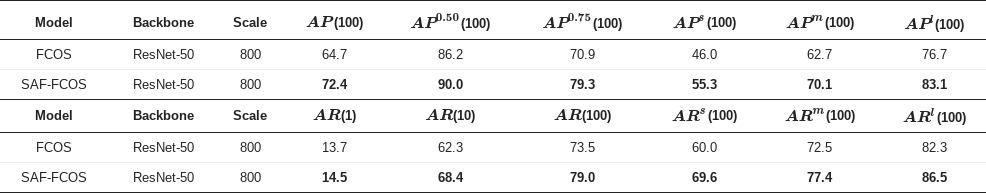
\includegraphics[width=\textwidth]{r2-hasil-2.png}
\end{frame}


\begin{frame}
    \frametitle{Pustaka 2: Kesimpulan}

    \large
    \textbf{Kelebihan}\\
    \normalsize
    \begin{itemize}
        \item Permodelan sistem lebih mudah karena fusion dilakukan di tingkat Fitur, tepat setelah ekstraksi fitur gambar dan radar.
    \end{itemize}

    \large
    \textbf{Kekurangan}\\
    \normalsize
    \begin{itemize}
        \item Permodelan di tingkat fitur menyebabkan Kamera dan Radar menjadi terkopel, sehingga keduanya harus bekerja dengan baik agar keluaran algoritma ini sesuai keinginan desain.
    \end{itemize}

    \large
    \textbf{Ide}\\
    \normalsize
    \begin{itemize}
        \item Metode deteksi gambar pada penelitian ini dapat digunakan sepenuhnya.
        \item Mencoba fusion di tingkat data.
        \item Menggunakan algoritma ini sebagai pembanding.
    \end{itemize}

\end{frame}
